\documentclass[11pt, oneside]{article}   	% use "amsart" instead of "article" for AMSLaTeX format
\usepackage[margin = 1in]{geometry}                		% See geometry.pdf to learn the layout options. There are lots.
\geometry{letterpaper}                   		% ... or a4paper or a5paper or ... 
%\geometry{landscape}                		% Activate for rotated page geometry
\usepackage[parfill]{parskip}    		% Activate to begin paragraphs with an empty line rather than an indent
\usepackage{graphicx, array}				% Use pdf, png, jpg, or eps§ with pdflatex; use eps in DVI mode
								% TeX will automatically convert eps --> pdf in pdflatex		
\usepackage{amssymb, enumerate, tikz, multicol}

%SetFonts

%SetFonts


\title{Math F113X: Homework Set 7}
%\author{The Author}
\date{}							% Activate to display a given date or no date

\begin{document}

\maketitle

\vspace{-1.5cm}


\fbox{\parbox{\textwidth}{

\begin{itemize}
\item Start with the introductory Problems A, B, and C.
\item Then complete problems \#19ac, 21, and 22ac from the Graph Theory section.
\item Next, complete Problems D and E.

\item Finally, answer the following {\bf reflection question}: What did you learn from checking your homework answers against the provided solutions?
\end{itemize}
}}

\vfill

\textbf{Problem A:} 
\begin{enumerate}
\item Write out what $5!$ means and find its value.
\item Expand $8.75 \times 10^8$
\item Write $35,200,000$ in scientific notation.
\item Go to WolframAlpha to compute $20!$ and write it in scientific notation, holding only the first three digits.\\
\end{enumerate}
\vfill

\textbf{Problem B:} This question is about notation of complete graphs and complete bipartite graphs.\\
	\begin{enumerate}
	\item We use $K_n$ to denote the \textbf{complete graph} on $n$ vertices. Draw $K_3$, $K_4,$ $K_5,$ and $K_6.$
	\item We use $K_{n,n}$ to denote the \textbf{balanced complete bipartite graph} on $2n$ vertices. Observe that $K_{2,2}$ and $K_{3,3}$ are drawn below. Draw $K_{4,4}.$\\
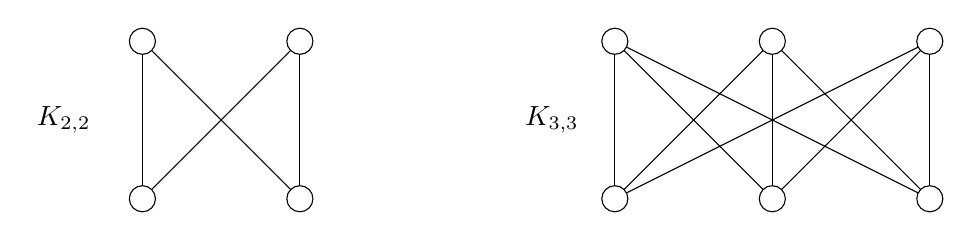
\begin{tikzpicture}[baseline=(current bounding box.center)]
\tikzstyle{vtx}=[circle, draw, fill=white,minimum size=2pt]
\node at (-1, 1){$K_{2,2}$};
\node at (5.2,1){$K_{3,3}$};
\tikzstyle{every node} = [vtx];
\foreach \i in {6,8,10}{
	\draw (6,0) -- (\i,2);
	\draw (8,0) -- (\i,2);
	\draw (10,0) -- (\i,2);}
\foreach \i in {0,2}{
	\draw (0,0) -- (\i,2);
	\draw (2,0) -- (\i,2);}
\foreach \i in {0,2,6,8,10}{
	\node  at (\i,0){};
	\node at (\i,2){};}
\end{tikzpicture}

	\item How many edges would $K_{10}$ have? How many edges would $K_{10,10}$ have?
	\item Give an example of a practical situation that could be modeled by a weighted $K_{10,10}$? (State what the vertices and edge weights represent.)\\
	\end{enumerate}
	
	\vfill
	
\textbf{Problem C:} Answer the questions about the graph below.\\
\begin{center}
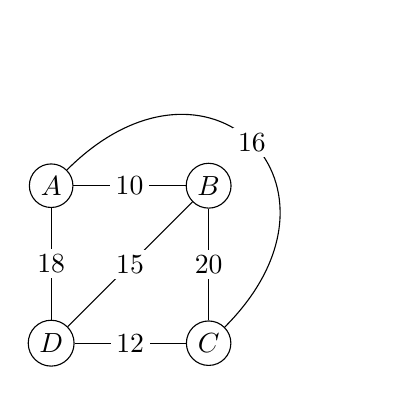
\begin{tikzpicture}[lbl/.style={inner sep = 2pt, fill = white}]
\tikzstyle{vtx}=[circle, draw, inner sep=2pt]
\node[vtx] (A) at (0,2){$A$};
\node[vtx] (B) at (2,2){$B$};
\node[vtx] (C) at (2,0){$C$};
\node[vtx] (D) at (0,0){$D$};
\foreach \i/\j/\k in {A/B/10,B/C/20,C/D/12,D/A/18,B/D/15}{\draw (\i) --node[lbl]{\k} (\j);}
\draw (A) .. controls (2,4) and (4,2) .. (C)
  node[pos=0.5,inner sep = 2pt, fill = white]{$16$};
\end{tikzpicture}
\end{center}

\begin{enumerate}
\item How many different Hamiltonian circuits are possible? (Assume that it doesn't matter what the starting vertex is.)
\item List all of Hamiltonian circuits and calculate their weight.
\item Using the list above, identify a circuit with the lowest total weight.
\item The steps above are those of what algorithm?
\item Using the work above, find a Hamiltonian \emph{path} of lowest total weight.
\end{enumerate}


%\textbf{Problem D:}
%\begin{enumerate} 
%\item For what values of $n$ does $K_n$ have an Euler circuit? 
%\item For what values of $n$ does $K_n$ have a Hamiltonian circuit? 
%\item For what values of $n$ does $K_{n,n}$ have an Euler circuit? 
%\item For what values of $n$ does $K_{n,n}$ have a Hamiltonian circuit? \\
%\end{enumerate}
\textbf{Problem D:} Suppose someone wants to visit the capital city of every state in the contiguous 48 states and Washington DC. So, they will visit 49 cities in total. [NOTE: you will need to use a computational tool, like WolframAlpha, to complete this problem.]
	\begin{enumerate}
	\item Suppose they want to start and end the 49-city-tour at the same place. How many different tours are possible? (Your answer should be in \emph{both} factorial notation and in scientific notation.)
	\item Suppose you have a computer that can calculate the length of 1000 49-city-tours in one second. How long would it take the computer to calculate the length of all possible 49-city-tours? Give your answer in \emph{years}. 
	\item What does your answer in part $2$ indicate about the Brute Force algorithm?
	\end{enumerate}
\textbf{Problem E:} Create weighted, 5-vertex graph with vertex set $A$, $B$, $C$, $D$, and $E,$ such that the Nearest Neighbor algorithm starting at $A$ will give an optimal solution but starting at $B$ will give the worst possible solution. Show your answer is correct. \\


\hrulefill

Remember to write up your homework solutions according to the homework writeup guidelines. 

Homework is graded using the following rubric for each problem (or problem part):

\begin{description}
\item[2 points:] You provided a complete answer, with supporting work, written up clearly
\item[1 point:] Some attempt at a solution, but incomplete writeup / unclear / illegible / no answer
\item[1 point:] Only an answer, with no supporting work 
\item[0 points:] Missing.
\end{description}

After you do the homework, you need to check your answers against the solutions! Then figure out your errors (if any) and revise your homework before you submit it. Finally, answer the reflection question.

Homework must be submitted on Gradescope.

\end{document}  